% !TeX program = pdflatex
% =============================================================================
% Arbeitsblatt: Kräfte (Teil 1) (nicht bewertet, Übungsmaterial für den Unterricht)
% Kantonsschule KFR -- Physik, 4. Klasse, 1. HS, Mechanik
%
% Kopiert aus vorlagen/arbeitsblatt-vorlage.tex und um dieselben
% Farb-/Boxdefinitionen ergänzt wie freier-fall-arbeitsblatt.tex /
% bewegungsgleichungen-arbeitsblatt.tex. Templates sind selbstständig/nicht
% DRY, siehe CLAUDE.md.
%
% Scope (siehe lernziele.md, Abschnitt "Abgrenzung"): allgemeiner Kraftbegriff,
% Vektorcharakter, Federkraftmesser-Messprinzip, Kraftarten OHNE Formel,
% Kräftebilder, grafisches/rechnerisches Addieren und Zerlegen von Kräften,
% Kräftegleichgewicht als Phänomen. Benannte Kraftarten MIT Formel
% (F_G = m*g, Federkraft, Normalkraft, Reibungskraft) sind bewusst NICHT Teil
% dieser Einheit (folgen in Kräfte Teil 2, nach den Newtonschen Gesetzen).
% Deshalb wird die Gewichtskraft in jeder Aufgabe direkt als Newton-Wert
% gegeben, nie über m*g berechnet, und die Komponente der Gewichtskraft
% senkrecht zur schiefen Ebene wird bewusst "Normalkomponente" (nicht
% "Normalkraft") genannt, um sie von der späteren Reaktionskraft der
% Unterlage (3. Newtonsches Axiom, noch nicht behandelt) abzugrenzen.
%
% Stand: Lernziele, Einleitung, Theorie und Aufgaben fertig. LZ-Nummerierung
% entspricht der Dokumentreihenfolge und stimmt mit lernziele.md überein
% (keine Umnummerierung nötig).
% =============================================================================
\documentclass[addpoints,11pt,a4paper]{exam}

\usepackage[T1]{fontenc}
\usepackage[utf8]{inputenc}
\usepackage[ngerman]{babel}
\usepackage{lmodern}
\usepackage[a4paper,margin=2.2cm,headheight=14pt]{geometry}
\usepackage{amsmath}
\usepackage{amssymb}
\usepackage{siunitx}
% Hausstil: zusammengesetzte Einheiten immer als echter Bruch (\frac), nicht
% als Schrägstrich inline oder \tfrac. Gilt global für jedes \si/\SI.
\sisetup{per-mode=fraction,fraction-command=\frac}
\usepackage{array,booktabs,tabularx,multirow}
\usepackage{enumitem}
\usepackage{graphicx}
\usepackage{xcolor}
\usepackage{colortbl}
\usepackage{tikz}
\usepackage{physics}
\usepackage{circuitikz}
\usepackage[most]{tcolorbox}
\usepackage{lastpage}

\usetikzlibrary{arrows.meta,calc,angles,quotes}

\setlength{\parindent}{0pt}
\setlength{\parskip}{0.45em}

% -----------------------------
% Farben (Hausfarbschema Physik KFR)
% -----------------------------
\definecolor{titleblue}{HTML}{183A6B}
\definecolor{accentblue}{HTML}{2E6F9E}
\definecolor{lightblue}{HTML}{EAF4FB}
\definecolor{verylightblue}{HTML}{F7FBFE}
\definecolor{lightgray}{HTML}{F4F6F8}
\definecolor{darkgray}{HTML}{4A4A4A}
% Für Diagramme mit zwei verschiedenen Kräften/Linien: titleblue (dunkles
% Blau) + accentorange (Orange) sind weit genug auseinander (auch in
% Graustufen/für Farbenblinde unterscheidbar).
\definecolor{accentorange}{HTML}{D9720C}
% Für Diagramme mit DREI Kräften/Linien: dritte Farbe, die sich sowohl von
% titleblue als auch von accentorange klar unterscheidet.
\definecolor{accentpurple}{HTML}{7B2D8E}
% Theorieblock: eigene Farbe (grün), damit er sich auf einen Blick von den
% blauen Lernziele-/Aufgaben-Boxen abhebt.
\definecolor{theorygreen}{HTML}{2E7D4F}
\definecolor{lighttheorygreen}{HTML}{EAF7EF}
% Gruppenarbeitbox: eigene Farbe (Petrol/Teal), damit Partner-/Gruppenarbeit
% sich auf einen Blick von normalen Einzelaufgaben (blau, taskbox) und vom
% Theorieblock (grün, theoriebox) abhebt.
\definecolor{groupteal}{HTML}{1B7F72}
\definecolor{lightgroupteal}{HTML}{E8F5F3}

% -----------------------------
% Spaltentypen
% -----------------------------
\newcolumntype{Y}{>{\centering\arraybackslash}X}
\newcolumntype{P}[1]{>{\raggedright\arraybackslash}p{#1}}

% -----------------------------
% Boxen
% -----------------------------
\newtcolorbox{titlebox}{
  enhanced,
  colback=titleblue,
  colframe=titleblue,
  boxrule=0pt,
  arc=3mm,
  left=3mm,right=3mm,top=3mm,bottom=3mm
}

% exam.cls rückt die questions-Liste um die Breite von "10." (plus \labelsep)
% ein (Platz für die Nummerierung "1.", "2." ...); wir messen dieselbe
% Distanz hier unabhängig nach.
\newlength{\aufgabenindent}
\settowidth{\aufgabenindent}{10.\hskip\labelsep}

\newtcolorbox{infobox}{
  enhanced,
  breakable,
  colback=lightblue,
  colframe=accentblue,
  boxrule=0.7pt,
  arc=2mm,
  left=5mm,right=5mm,top=2mm,bottom=2mm
}

% theoriebox: wie infobox, aber grün und mit farbigem Titelbalken. Regel:
% hervorgehobene/definierte Begriffe INNERHALB einer theoriebox immer mit
% \textbf{\emph{...}} setzen (fett UND kursiv).
\newtcolorbox{theoriebox}[1][Theorie]{
  enhanced,
  breakable,
  colback=lighttheorygreen,
  colframe=theorygreen,
  title={#1},
  fonttitle=\bfseries,
  boxrule=0.7pt,
  arc=2mm,
  left=5mm,right=5mm,top=2mm,bottom=2mm
}

% taskbox steht direkt in der questions-Liste (vor dem ersten \question),
% also innerhalb von deren Einrückung.
\newtcolorbox{taskbox}[1][]{
  enhanced,
  breakable,
  colback=verylightblue,
  colframe=accentblue,
  title={#1},
  fonttitle=\bfseries,
  boxrule=0.7pt,
  arc=2mm,
  enlarge left by=-\aufgabenindent,
  width=\textwidth,
  left=5mm,right=5mm,top=2mm,bottom=2mm
}

% beispielbox: wie taskbox (blau), aber ausserhalb von questions, deshalb
% KEINE Einrückungskorrektur nötig.
\newtcolorbox{beispielbox}[1][Beispiel]{
  enhanced,
  breakable,
  colback=verylightblue,
  colframe=accentblue,
  title={#1},
  fonttitle=\bfseries,
  boxrule=0.7pt,
  arc=2mm,
  left=5mm,right=5mm,top=2mm,bottom=2mm
}

% Regel für groupbox: JEDE Aufgabe, bei der Schülerinnen/Schüler zu zweit
% oder in einer Gruppe zusammenarbeiten, bekommt diese Box statt der blauen
% taskbox. Strukturell identisch zu taskbox.
\newtcolorbox{groupbox}[1][Gruppenarbeit]{
  enhanced,
  breakable,
  colback=lightgroupteal,
  colframe=groupteal,
  title={#1},
  fonttitle=\bfseries,
  boxrule=0.7pt,
  arc=2mm,
  enlarge left by=-\aufgabenindent,
  width=\textwidth,
  left=5mm,right=5mm,top=2mm,bottom=2mm
}

% hinweisbox: eigene Farbe (Orange), für wichtige Klarstellungen/Warnungen
% vor häufigen Verwechslungen. Steht wie infobox/theoriebox/beispielbox
% ausserhalb von questions, KEINE Einrückungskorrektur nötig.
\definecolor{lightorange}{HTML}{FCEEE0}
\newtcolorbox{hinweisbox}[1][Hinweis]{
  enhanced,
  breakable,
  colback=lightorange,
  colframe=accentorange,
  title={#1},
  fonttitle=\bfseries,
  boxrule=0.7pt,
  arc=2mm,
  left=5mm,right=5mm,top=2mm,bottom=2mm
}

\newtcolorbox{answerbox}{
  breakable,
  colback=white,
  colframe=gray!55,
  boxrule=0.5pt,
  arc=1.5mm,
  left=2mm,right=2mm,top=2mm,bottom=2mm
}

% --- Lösungen ein-/ausblenden -----------------------------------------------
% Schülerexemplar (Standard): \noprintanswers
% Lehrer-/Lösungsexemplar:    \printanswers
\noprintanswers
% \printanswers

% --- Punkte bleiben intern, werden aber nicht gedruckt ----------------------
\pointformat{}

% --- Lösungsbox auf Deutsch, farblich abgesetzt -----------------------------
\renewcommand{\solutiontitle}{\noindent\color{titleblue}\textbf{Lösung:}\enspace}

% --- Kopf-/Fusszeile: Thema/Titel oben, Seitenzahl unten --------------------
\pagestyle{headandfoot}
\cfoot{\textcolor{darkgray}{Seite \thepage\ von \pageref{LastPage}}}

% --- Kopfzeile: Klasse / Datum / Thema / Titel ------------------------------
\newcommand{\Kopfzeile}[4]{%
  \begin{titlebox}
    {\color{white}\sffamily\bfseries\Large #4}
  \end{titlebox}
  \vspace{0.5em}
  \noindent\textbf{Klasse:}~#1 \hfill \textbf{Datum:}~#2 \hfill \textbf{Thema:}~#3
    \hfill \textbf{Lehrperson:}~Loris Keller
  \vspace{0.8em}
  \lhead{\textcolor{darkgray}{#3}}
  \rhead{\textcolor{darkgray}{#4}}
}

% --- Antwortraum: ca. 2.5 cm Platz pro Punkt, als umrandetes Feld -----------
\newlength{\antwortraumlen}
\newcommand{\Antwortraum}[1]{%
  \pgfmathsetlength{\antwortraumlen}{#1*2.5cm}%
  \begin{answerbox}
    \rule{0pt}{\antwortraumlen}%
  \end{answerbox}%
}

% Werte für Kopfzeile zentral setzen
\newcommand{\Klasse}{4a}
\newcommand{\Datum}{TT.MM.JJJJ}
\newcommand{\Thema}{Kräfte (Teil 1)}
\newcommand{\ArbeitsblattTitel}{Arbeitsblatt: Kräfte (Teil 1)}

\begin{document}

\Kopfzeile{\Klasse}{\Datum}{\Thema}{\ArbeitsblattTitel}

% --- Lernziele: aus lernziele.md (Backward-Design, Stufe 1) übernommen.
% LZ1..LZ8 entsprechen der Reihenfolge, in der die zugehörigen
% Theorieboxen/Übungen im Dokument erscheinen; das stimmt hier mit der
% ursprünglichen Backward-Design-Reihenfolge überein, keine Umnummerierung
% nötig. -----------------------------------------------------------------
\begin{infobox}
\textbf{Lernziele}\\
Am Ende dieser Einheit kann ich \dots
\begin{itemize}[leftmargin=1.2cm,itemsep=0.25em]
  \item Kräfte an ihren Wirkungen erkennen und zwischen Bewegungsänderung, Verformung und Spannungsänderung unterscheiden. (LZ1)
  \item den physikalischen Kraftbegriff (Vektor mit Betrag, Richtung, Angriffspunkt; Einheit Newton) vom alltagssprachlichen Verständnis abgrenzen. (LZ2)
  \item Kräfte in verschiedenen Vorsätzen (mN, cN, N, kN, MN) angeben und umrechnen.
  \item das Messprinzip eines Federkraftmessers erklären. (LZ3)
  \item gängige Kraftarten benennen und in Kontakt- und Nicht-Kontaktkräfte einteilen. (LZ4)
  \item erklären, dass sich alle Kräfte auf vier fundamentale Kräfte zurückführen lassen, und einer Alltagskraft die passende fundamentale Kraft zuordnen.
  \item Kräfte mit Betrag, Richtung und Angriffspunkt in einem Kräftebild darstellen. (LZ5)
  \item mehrere Kräfte grafisch und rechnerisch zu einer resultierenden Kraft addieren. (LZ6)
  \item eine Kraft in zwei Komponenten zerlegen, insbesondere an der schiefen Ebene mit Trigonometrie. (LZ7)
  \item Kräfte mit Lineal, Geodreieck und Massstab addieren, subtrahieren und zerlegen.
  \item erklären, dass Ruhe eines Körpers Kräftegleichgewicht (nicht Kräftefreiheit) bedeuten kann, und einfache Gleichgewichtssituationen im Kräftebild untersuchen. (LZ8)
\end{itemize}
\end{infobox}

% --- Einleitung: Fussballschuss-Hook, direkt aus lernziele.md übernommen.
% Bild bereits vorhanden: Bilder/Fussball_Schuss.jpeg. Bewusst noch keine
% Erwähnung von Richtung/Verformung/Angriffspunkt im Einleitungstext selbst
% (folgt in der Think-Pair-Share-Box direkt danach). ------------------------
\begin{beispielbox}[Einleitung: Der schnellste Torschuss der Fussballgeschichte]
\begin{center}
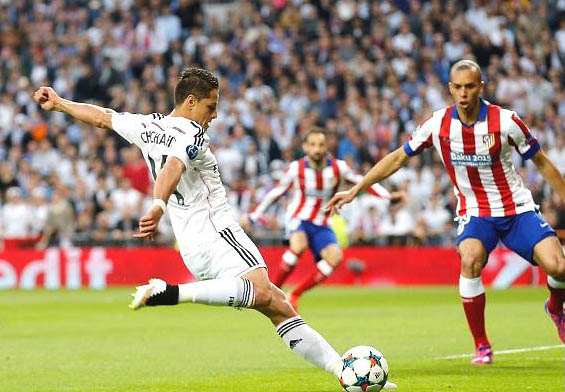
\includegraphics[width=0.55\linewidth]{Bilder/Fussball_Schuss.jpeg}
\end{center}
{\scriptsize Der Moment, in dem der Fuss bei einem Torschuss den Ball
berührt: genau in diesem Sekundenbruchteil wirkt eine sehr grosse Kraft.}

Am 16. September 1996 schoss der englische Fussballspieler David Hirst
(Sheffield Wednesday) im Spiel gegen Arsenal einen Ball mit rund
\SI{183}{\kilo\meter\per\hour} gegen die Querlatte, gemessen aus
\SI{13.5}{\meter} Distanz zum Tor. Bis heute gilt das als der schnellste
offiziell gemessene Torschuss der englischen ersten Liga (Guinness World
Records).

Rechnet man diesen Schuss in eine Kraft um (Ballmasse etwa
\SI{0.43}{\kilo\gram}, Kontaktzeit zwischen Fuss und Ball etwa
\SI{10}{\milli\second}), ergibt sich ein Wert von rund \SI{2200}{\newton}. Das entspricht ungefähr
dem Gewicht von \SI{220}{\kilo\gram}, gut dem 500-Fachen der Gewichtskraft
des Balls selbst. Und das alles in einem Zeitraum, der viel kürzer ist als
ein Wimpernschlag.
\end{beispielbox}

% --- Think-Pair-Share direkt im Anschluss an den Hook, wie in lernziele.md
% vorgeschlagen (Sandwich-Methode C3). Adressiert Lernschwierigkeit 1
% (Kraft als vager Clusterbegriff), indem die SuS die Wirkungen einer Kraft
% zuerst selbst formulieren, bevor die Theoriebox sie unten formalisiert. ---
\begin{groupbox}[Think-Pair-Share: Was passiert in diesem Moment?]
\textbf{Denkfrage:} Was passiert mit Ball und Fuss in dem Moment, in dem sie
sich berühren, und woran erkennst du, dass hier eine Kraft wirkt?

\begin{parts}
  \part[2] \textbf{Think:} Notiere deine eigene Antwort still für dich,
  bevor du mit jemandem sprichst.
  \Antwortraum{2}

  \part[1] \textbf{Pair:} Vergleiche deine Antwort zu zweit mit deiner
  Sitznachbarin oder deinem Sitznachbarn. Wo stimmt ihr überein, wo nicht?
  \Antwortraum{1}

  \part[1] \textbf{Share:} Seid bereit, eure gemeinsame Antwort der Klasse
  kurz vorzustellen.
\end{parts}
\end{groupbox}

% =============================================================================
% Theorie: fachliche Grundlage für die Aufgaben, in eigene Boxen unterteilt
% (je Unterthema eine theoriebox), Reihenfolge = Lernzielreihenfolge oben.
% =============================================================================
\begin{theoriebox}[Die drei Wirkungen einer Kraft]
Eine Kraft lässt sich nicht direkt sehen, nur an dem erkennen, was sie
bewirkt. Man unterscheidet drei grundsätzliche \textbf{\emph{Wirkungen
einer Kraft}}:

\begin{itemize}[leftmargin=1.2cm,itemsep=0.35em]
  \item \textbf{\emph{Bewegungsänderung}}: Ein Körper wird schneller,
  langsamer, oder seine Bewegungsrichtung ändert sich. Beispiel: Ein Auto
  beschleunigt, sobald der Motor eine Kraft auf die Räder ausübt.
  \item \textbf{\emph{Verformung}}: Die Form eines Körpers ändert sich.
  Beispiel: Ein Fussball wird im Moment des Torschusses kurz zusammengedrückt
  (siehe Einleitung oben).
  \item \textbf{\emph{Spannungsänderung}}: Im Inneren eines Materials
  ändert sich die mechanische Spannung, ohne dass von aussen unbedingt eine
  Verformung oder Bewegung sichtbar sein muss. Beispiel: Ein gespanntes
  Trampolintuch oder eine gespannte Bogensehne.
\end{itemize}

Oft treten mehrere dieser Wirkungen gleichzeitig auf: Beim Fussballschuss
aus der Einleitung wird der Ball sowohl verformt (Verformung) als auch
beschleunigt (Bewegungsänderung).
\end{theoriebox}

\begin{theoriebox}[Der physikalische Kraftbegriff]
Im Alltag wird das Wort \glqq Kraft\grqq{} sehr unterschiedlich verwendet,
zum Beispiel als Muskelkraft, als \glqq Willenskraft\grqq{}, oder wenn
jemand sagt \glqq nach dem Rennen hatte er keine Kraft mehr\grqq{}. Dabei
vermischt sich der Alltagsbegriff oft mit ganz anderen physikalischen
Grössen wie Energie, Geschwindigkeit oder Ausdauer.

Physikalisch ist eine \textbf{\emph{Kraft}} eine \textbf{\emph{Vektorgrösse}}:
Sie ist erst dann vollständig beschrieben, wenn drei Dinge bekannt sind:
\begin{itemize}[leftmargin=1.2cm,itemsep=0.25em]
  \item der \textbf{\emph{Betrag}} (wie stark die Kraft ist), Einheit
  $\si{\newton}$ (Kurzzeichen $\text{N}$),
  \item die \textbf{\emph{Richtung}} (in welche Richtung sie wirkt),
  \item der \textbf{\emph{Angriffspunkt}} (an welcher Stelle des Körpers sie
  wirkt).
\end{itemize}
Formelzeichen: $F$. Eine einzelne Zahl (nur der Betrag) reicht deshalb nie
aus, um eine Kraft vollständig zu beschreiben.

Zur Grössenordnung: $\SI{1}{\newton}$ entspricht ungefähr der
Gewichtskraft einer kleinen Tafel Schokolade (etwa \SI{100}{\gram}) hier auf
der Erde.
\end{theoriebox}

\begin{hinweisbox}[Hinweis: Kraft ist nicht dasselbe wie \dots]
\glqq Kraft\grqq{} ist im Alltag ein sehr weiter, unscharfer Begriff und wird
oft mit anderen physikalischen Grössen verwechselt. Kraft ist
\textbf{nicht} dasselbe wie \emph{Geschwindigkeit} (wie schnell sich etwas
bewegt), \emph{Energie} (wie viel ein Körper \glqq leisten\grqq{} kann,
bevor er \glqq erschöpft\grqq{} ist) oder \emph{Impuls} (Produkt aus Masse
und Geschwindigkeit). Ein Sprinter, der am Ende eines Rennens erschöpft
ist, hat keine \glqq Energie mehr übrig\grqq{}, aber er übt in diesem
Moment trotzdem weiterhin physikalische Kräfte aus (siehe Clicker-Aufgabe
weiter unten).
\end{hinweisbox}

\begin{theoriebox}[Grössenordnungen: Vorsätze für Newton]
Kräfte kommen in der Natur und im Alltag in ganz unterschiedlichen
Grössenordnungen vor: von der winzigen Gewichtskraft eines Reiskorns bis
zur gewaltigen Schubkraft einer Rakete. Damit man nicht ständig sehr
kleine oder sehr grosse Zahlen vor die Einheit $\si{\newton}$ schreiben
muss, verwendet man dieselben \textbf{\emph{SI-Vorsätze}}, die du schon
von anderen Grössen kennst (z.\,B. Millimeter, Kilogramm):

\begin{center}
\begin{tabular}{@{}lllp{5.3cm}@{}}
\toprule
\textbf{Vorsatz} & \textbf{Symbol} & \textbf{Faktor} & \textbf{Typisches Beispiel} \\
\midrule
Milli- & $\si{\milli\newton}$ & $10^{-3}\,\si{\newton}$ & Gewichtskraft eines Reiskorns ($\approx\SI{0.25}{\milli\newton}$) \\
Centi- & $\si{\centi\newton}$ & $10^{-2}\,\si{\newton}$ & Gewichtskraft einer 5-Rappen-Münze ($\approx\SI{1.8}{\centi\newton}$) \\
(keiner) & $\si{\newton}$ & $10^{0}\,\si{\newton}$ & Gewichtskraft einer Tafel Schokolade ($\approx\SI{1}{\newton}$) \\
Kilo- & $\si{\kilo\newton}$ & $10^{3}\,\si{\newton}$ & Gewichtskraft eines Kleinwagens ($\approx\SI{12}{\kilo\newton}$) \\
Mega- & $\si{\mega\newton}$ & $10^{6}\,\si{\newton}$ & Schubkraft einer Rakete beim Start ($\approx\SI{7.6}{\mega\newton}$, Falcon 9) \\
\bottomrule
\end{tabular}
\end{center}

Zum Umrechnen gilt wie bei jedem SI-Vorsatz: Ein Schritt nach rechts in
der Tabelle bedeutet, mit $1000$ zu multiplizieren (bzw. bei Centi-
zwischendrin mit $100$); ein Schritt nach links bedeutet, durch denselben
Faktor zu dividieren. Zum Beispiel:
\[
  \SI{1}{\newton} = \SI{1000}{\milli\newton}, \qquad
  \SI{1}{\kilo\newton} = \SI{1000}{\newton}, \qquad
  \SI{1}{\centi\newton} = \SI{10}{\milli\newton} = \SI{0.01}{\newton}.
\]

\textbf{Wann welcher Vorsatz sinnvoll ist:} Millinewton und Centinewton
eignen sich für sehr kleine Kräfte (Insekten, Papier, kleine
Federkraftmesser im Biologieunterricht), Kilonewton und Meganewton für
sehr grosse Kräfte (Fahrzeuge, Bauwerke, Raketen). Für die meisten Kräfte, mit
denen du im Alltag direkt zu tun hast (ein Buch heben, eine Tür
aufdrücken), reicht die Einheit Newton selbst völlig aus.
\end{theoriebox}

\begin{questions}
\begin{taskbox}[Übung: Newton umrechnen]
\question[8] Rechne die folgenden Kräfte in die jeweils verlangte
Einheit um.

\begin{parts}
  \part[2] Der Fussballschuss aus der Einleitung übt eine Kraft von
  $\SI{2200}{\newton}$ aus. Gib diese Kraft in $\si{\kilo\newton}$ an.
  \Antwortraum{2}
  \begin{solution}
  \[
    \SI{2200}{\newton} = \SI{2.2}{\kilo\newton}.
  \]
  \end{solution}

  \part[2] Eine Ameise hat eine Gewichtskraft von etwa
  $\SI{0.2}{\milli\newton}$. Gib diese Kraft in $\si{\newton}$ an.
  \Antwortraum{2}
  \begin{solution}
  \[
    \SI{0.2}{\milli\newton} = \SI{0.0002}{\newton}.
  \]
  \end{solution}

  \part[2] Ein Baukran hebt eine Last mit einer Kraft von
  $\SI{45}{\kilo\newton}$. Gib diese Kraft in $\si{\newton}$ an.
  \Antwortraum{2}
  \begin{solution}
  \[
    \SI{45}{\kilo\newton} = \SI{45000}{\newton}.
  \]
  \end{solution}

  \part[2] Ordne der Grösse nach, von klein nach gross: die Gewichtskraft
  eines Reiskorns ($\SI{0.25}{\milli\newton}$), eines Kleinwagens
  ($\SI{12}{\kilo\newton}$), einer Tafel Schokolade ($\SI{1}{\newton}$)
  und einer 5-Rappen-Münze ($\SI{1.8}{\centi\newton}$).
  \Antwortraum{2}
  \begin{solution}
  Alle in Newton umgerechnet: Reiskorn $\SI{0.00025}{\newton}$, Münze
  $\SI{0.018}{\newton}$, Schokolade $\SI{1}{\newton}$, Kleinwagen
  $\SI{12000}{\newton}$. Reihenfolge: Reiskorn $<$ Münze $<$ Schokolade
  $<$ Kleinwagen.
  \end{solution}
\end{parts}
\end{taskbox}
\end{questions}

\begin{theoriebox}[Das Messprinzip des Federkraftmessers]
Ein \textbf{\emph{Federkraftmesser}} (auch Kraftmesser genannt) nutzt eine
einfache Beobachtung: Je stärker eine Kraft an einer Feder zieht, desto
weiter dehnt sich die Feder. Zieht man doppelt so stark, dehnt sich die
Feder doppelt so weit; die Dehnung ist also proportional zur ziehenden
Kraft.

Diese Proportionalität macht die Feder zu einem Messinstrument: Man hängt
den zu messenden Gegenstand an die Feder, liest die Dehnung an einer
Skala ab, und diese Skala ist bereits direkt in $\si{\newton}$ geeicht
(kalibriert), sodass man den Kraftbetrag ohne Umrechnung ablesen kann.

\begin{center}
\begin{minipage}{0.38\linewidth}\centering
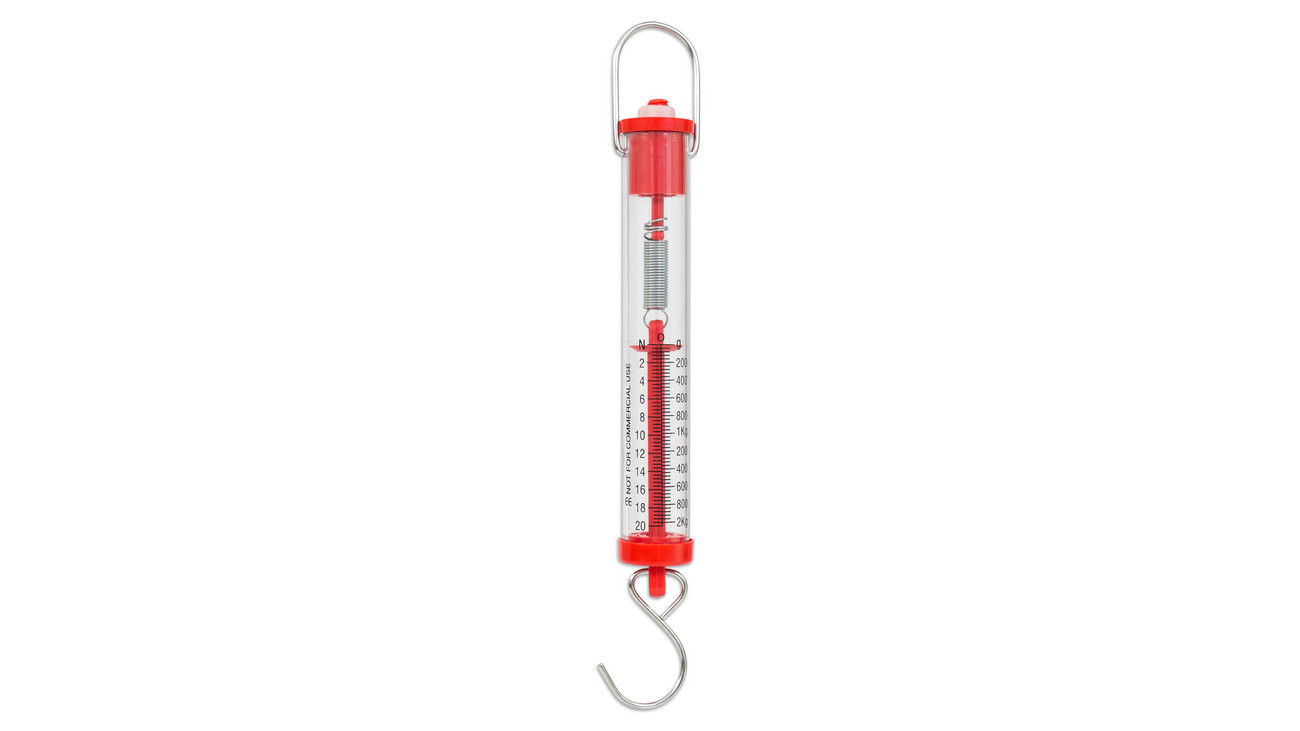
\includegraphics[width=0.7\linewidth]{Bilder/Federwaage.jpg}\\[0.2em]
{\scriptsize Ein echter Federkraftmesser: rot die Feder im
durchsichtigen Gehäuse, links die in Newton geeichte Skala.}
\end{minipage}\hfill
\begin{minipage}{0.55\linewidth}\centering
\begin{tikzpicture}[scale=0.9]
  % Gehäuse
  \draw[thick] (0,3.2) -- (-0.5,3.2) -- (-0.5,2.9) -- (0,2.9);
  \draw[thick,fill=lightgray] (-0.35,1.2) rectangle (0.35,3.2);
  \foreach \y in {1.5,1.9,2.3,2.7} {
    \draw (-0.35,\y) -- (0.35,\y);
  }
  \node[right] at (0.4,2.7) {\scriptsize \SI{40}{\newton}};
  \node[right] at (0.4,2.3) {\scriptsize \SI{30}{\newton}};
  \node[right] at (0.4,1.9) {\scriptsize \SI{20}{\newton}};
  \node[right] at (0.4,1.5) {\scriptsize \SI{10}{\newton}};
  % Feder (Zickzack) von Gehäuse bis Zeiger
  \draw[thick,titleblue] (0,2.9) -- (0.15,2.65) -- (-0.15,2.4) -- (0.15,2.15) -- (-0.15,1.9) -- (0,1.8);
  \draw[thick] (0,1.8) -- (0,1.2);
  % Haken und Gewicht
  \draw[thick] (0,1.2) -- (0,0.9);
  \draw[thick,fill=accentorange!30] (-0.3,0.9) rectangle (0.3,0.5);
  \node at (0,0.7) {\scriptsize $F$};
\end{tikzpicture}\\[0.2em]
{\scriptsize Schema: Die Dehnung der Feder ist proportional zur
ziehenden Kraft $F$, die Skala ist direkt in Newton geeicht.}
\end{minipage}
\end{center}
\end{theoriebox}

\begin{questions}
\begin{taskbox}[Übung: Federkraftmesser verstehen]
\question[3] Ein Federkraftmesser zeigt bei einer Kraft von $\SI{5}{\newton}$
eine Dehnung von $\SI{2}{\centi\meter}$.

\begin{parts}
  \part[3] Wie weit dehnt sich dieselbe Feder bei einer Kraft von
  $\SI{15}{\newton}$? Begründe mit dem Messprinzip aus der Theoriebox.
  \Antwortraum{3}
  \begin{solution}
  Die Dehnung ist proportional zur Kraft. $\SI{15}{\newton}$ ist die
  dreifache Kraft von $\SI{5}{\newton}$, deshalb ist auch die Dehnung
  dreifach so gross: $3\cdot\SI{2}{\centi\meter} = \SI{6}{\centi\meter}$.
  \end{solution}
\end{parts}
\end{taskbox}
\end{questions}

% --- Plenum: Vorwissen aktivieren, bevor die Kraftarten formal eingefuehrt
% werden (Sandwich-Methode, analog zu C1 Sortieraufgabe/B1
% Vergewisserungsphase, hier als Klassengespraech statt Einzel-/Partnerarbeit).
\begin{questions}
\begin{taskbox}[Plenum: Kraftarten sammeln]
\question[4] Sammelt gemeinsam als Klasse (im Plenum), welche Kraftarten
euch bereits bekannt sind oder einfallen, sei es aus dem Alltag, aus
anderen Fächern (z.\,B. Biologie, Chemie) oder aus den Medien. Die
Lehrperson sammelt eure Vorschläge an der Tafel.

\begin{parts}
  \part[4] Notiere hier die an der Tafel gesammelte Liste für dich.
  \Antwortraum{4}
  \begin{solution}
  Mögliche Nennungen (die tatsächliche Liste der Klasse darf davon
  abweichen oder mehr enthalten): Muskelkraft, Reibungskraft,
  Zugkraft/Seilkraft, Normalkraft, Federkraft, Auftriebskraft,
  Gewichtskraft/Gravitationskraft, elektrische Kraft, magnetische Kraft,
  Windkraft, Wasserkraft (Strömung), Motorkraft/Antriebskraft,
  Bremskraft.
  \end{solution}
\end{parts}
\end{taskbox}
\end{questions}

\begin{theoriebox}[Kraftarten: Kontakt- und Nicht-Kontaktkräfte]
Kräfte lassen sich danach einteilen, ob ein direkter Kontakt zwischen den
beteiligten Körpern nötig ist:

\begin{itemize}[leftmargin=1.2cm,itemsep=0.3em]
  \item \textbf{\emph{Kontaktkräfte}} (die Körper berühren sich):
  Muskelkraft, Zugkraft (z.\,B. an einem Seil), Reibungskraft, Normalkraft
  (Kraft einer Unterlage), Federkraft, Auftriebskraft in Wasser oder Luft.
  \item \textbf{\emph{Nicht-Kontaktkräfte}} (wirken auch ohne Berührung,
  \glqq Fernwirkung\grqq{}): Gravitationskraft/Gewichtskraft, elektrische
  Kraft, magnetische Kraft.
\end{itemize}

In dieser Einheit lernst du diese Kraftarten zunächst nur mit Namen und
Beispiel kennen. Wie sich ihr jeweiliger Betrag berechnen lässt (zum
Beispiel die Gewichtskraft aus der Masse), ist Thema von Kräfte (Teil 2).
\end{theoriebox}

\begin{theoriebox}[Woher kommen all diese Kräfte? Die vier fundamentalen Kräfte]
Die Liste aus dem Plenum wirkt vielleicht lang und unübersichtlich. Die
gute Nachricht: Die Physik hat herausgefunden, dass sich
\textbf{\emph{alle}} Kräfte im Universum letztlich auf nur \textbf{\emph{vier
fundamentale Kräfte}} zurückführen lassen.

\begin{center}
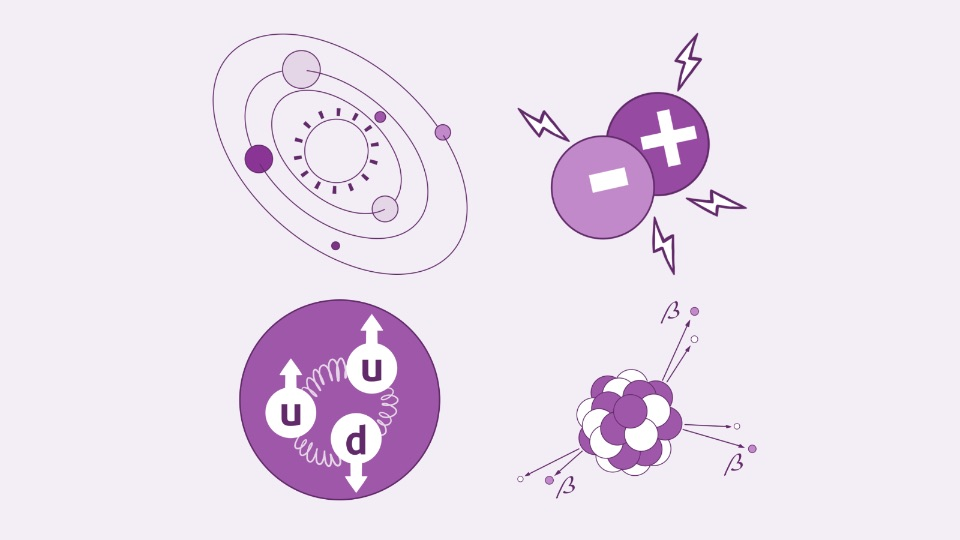
\includegraphics[width=0.75\linewidth]{Bilder/Fundamentale_Kraefte.jpg}\\[0.2em]
{\scriptsize Die vier fundamentalen Kräfte, symbolisch dargestellt: oben
links Gravitation, oben rechts Elektromagnetismus, unten links starke
Kernkraft (hält Quarks im Proton zusammen), unten rechts schwache
Kernkraft (verursacht Beta-Zerfall).}
\end{center}

\begin{itemize}[leftmargin=1.2cm,itemsep=0.3em]
  \item \textbf{\emph{Gravitation}}: wirkt zwischen allen Massen. Die
  \textbf{\emph{Gravitationskraft}} bzw. \textbf{\emph{Gewichtskraft}} aus
  der Liste \textbf{ist} bereits diese fundamentale Kraft selbst, nicht
  von ihr abgeleitet.
  \item \textbf{\emph{Elektromagnetismus}}: wirkt zwischen elektrischen
  Ladungen (und, eng damit verwandt, zwischen magnetischen Polen). Die
  \textbf{\emph{elektrische}} und die \textbf{\emph{magnetische Kraft}}
  aus der Liste sind ebenfalls direkt diese fundamentale Kraft.
  Erstaunlicherweise sind aber auch fast \textbf{\emph{alle
  Kontaktkräfte}} aus der Liste (Muskelkraft, Reibungskraft, Normalkraft,
  Federkraft, Zugkraft, Auftriebskraft) letztlich elektromagnetisch: Wenn
  sich zwei Oberflächen \glqq berühren\grqq{}, kommen sich ihre Atome nie
  wirklich vollständig nahe, sondern die negativ geladenen
  Elektronenhüllen der Atome stossen sich gegenseitig elektromagnetisch
  ab. Das, was sich wie \glqq Kontakt\grqq{} anfühlt, ist auf atomarer
  Ebene also nichts anderes als elektromagnetische Abstossung.
  \item \textbf{\emph{Starke Kernkraft}}: hält Protonen und Neutronen im
  Atomkern zusammen und überwindet dabei die elektrische Abstossung
  zwischen den positiv geladenen Protonen. Ohne sie gäbe es keine
  stabilen Atomkerne und damit keine Materie, wie wir sie kennen.
  \item \textbf{\emph{Schwache Kernkraft}}: verantwortlich für bestimmte
  radioaktive Zerfälle (z.\,B. Beta-Zerfall, bei dem sich ein Neutron in
  ein Proton umwandelt).
\end{itemize}

Starke und schwache Kernkraft wirken beide nur auf extrem kurze
Distanzen, innerhalb des Atomkerns. Sie erzeugen deshalb keine der
Alltagskräfte aus unserer gesammelten Liste, sind aber trotzdem
fundamental wichtig: Ohne die starke Kernkraft gäbe es überhaupt keine
Atome, aus denen alles andere besteht.
\end{theoriebox}

\begin{questions}
\begin{taskbox}[Clicker-ConcepTest: Kraft oder Erschöpfung?]
\question[6] \glqq Der Sprinter hat am Ende des Rennens keine Kraft mehr.
\grqq{} Stimmt diese Aussage aus physikalischer Sicht?

\begin{parts}
  \part[3] Kreuze die richtige Aussage an und begründe sie in ein bis zwei
  Sätzen.
  \begin{itemize}[leftmargin=1.2cm,itemsep=0.15em]
    \item[$\square$] A: Stimmt. Seine Muskeln sind leer, also kann er auch
    keine Kraft mehr ausüben.
    \item[$\square$] B: Stimmt nicht. Physikalisch bedeutet \glqq Kraft\grqq{}
    etwas anderes als \glqq Erschöpfung\grqq{}; der Sprinter übt weiterhin
    Kräfte aus (z.\,B. beim Auftreten auf den Boden), ist aber müde.
    \item[$\square$] C: Stimmt nicht, weil er am Ende des Rennens noch
    Geschwindigkeit hat.
  \end{itemize}
  \Antwortraum{2}
  \begin{solution}
  Richtig ist \textbf{B}. Die alltagssprachliche \glqq Kraft\grqq{}
  (Erschöpfung, verbrauchte Energie) ist nicht dasselbe wie die
  physikalische Kraft (Vektorgrösse mit Betrag, Richtung, Angriffspunkt).
  Auch ein erschöpfter Sprinter übt beim Laufen weiterhin Kräfte aus.
  Aussage A verwechselt Kraft mit Energie/Ausdauer, Aussage C verwechselt
  Kraft mit Geschwindigkeit, beides häufige Alltagsvorstellungen.
  \end{solution}

  \part[3] Nenne zwei Kontaktkräfte und eine Nicht-Kontaktkraft, die
  während des Laufens auf den Sprinter wirken könnten.
  \Antwortraum{3}
  \begin{solution}
  Kontaktkräfte (Beispiele): Reibungskraft zwischen Schuhen und Boden,
  Muskelkraft. Nicht-Kontaktkraft: Gewichtskraft (wirkt ununterbrochen,
  auch ohne Bodenkontakt in der Flugphase eines Schritts).
  \end{solution}
\end{parts}
\end{taskbox}
\end{questions}

\begin{theoriebox}[Kräftebilder zeichnen]
Um eine Kraft zeichnerisch darzustellen, verwendet man einen Pfeil und
beachtet dabei alle drei Eigenschaften einer Kraft (siehe Theoriebox oben):

\begin{enumerate}[leftmargin=1.2cm,itemsep=0.25em]
  \item Der \textbf{\emph{Angriffspunkt}} ist der Startpunkt des Pfeils.
  \item Die \textbf{\emph{Richtung}} des Pfeils entspricht der
  Wirkrichtung der Kraft.
  \item Die \textbf{\emph{Länge}} des Pfeils ist proportional zum
  \textbf{\emph{Betrag}} der Kraft, gemäss einem vorher festgelegten
  Massstab (z.\,B. $\SI{1}{\centi\meter} \,\widehat{=}\, \SI{10}{\newton}$).
\end{enumerate}

Diese Darstellung nennt man ein \textbf{\emph{Kräftebild}}. Ein Beispiel:
Auf einen Wagen wirkt eine Zugkraft $F_1=\SI{50}{\newton}$ nach rechts und
eine Reibungskraft $F_2=\SI{20}{\newton}$ nach links, beide mit
Angriffspunkt in der Wagenmitte, Massstab
$\SI{1}{\centi\meter}\,\widehat{=}\,\SI{10}{\newton}$:

\begin{center}
\begin{tikzpicture}[scale=1]
  \draw[thick,fill=lightgray] (-0.6,0) rectangle (0.6,0.6);
  \filldraw[black] (0,0.3) circle (1pt);
  \draw[->,thick,titleblue] (0,0.3) -- (5,0.3) node[midway,above] {\scriptsize $F_1=\SI{50}{\newton}$};
  \draw[->,thick,accentorange] (0,0.3) -- (-2,0.3) node[pos=0.75,above] {\scriptsize $F_2=\SI{20}{\newton}$};
\end{tikzpicture}\\[0.2em]
{\scriptsize Kräftebild eines Wagens: Beide Pfeile beginnen am selben
Angriffspunkt, ihre Länge entspricht dem gewählten Massstab.}
\end{center}
\end{theoriebox}

\begin{hinweisbox}[Hinweis: Häufiger Fehler beim Zeichnen]
Ein Kraftpfeil ist \textbf{keine} Bewegungsbahn: Er zeigt nicht, wohin sich
ein Körper bewegen \emph{wird}, sondern in welche Richtung die Kraft in
diesem Moment wirkt. Ausserdem muss die Länge tatsächlich zum gewählten
Massstab passen, zwei gleich lange Pfeile dürfen also nur dann gezeichnet
werden, wenn die beiden Kraftbeträge wirklich gleich gross sind.
\end{hinweisbox}

\begin{questions}
\begin{taskbox}[Übung: Kräftebild zeichnen]
\question[4] Auf eine Kiste wirkt eine Zugkraft $F_1=\SI{60}{\newton}$
nach rechts und eine Reibungskraft $F_2=\SI{30}{\newton}$ nach links, beide
mit Angriffspunkt in der Kistenmitte.

\begin{parts}
  \part[4] Zeichne das Kräftebild mit dem Massstab
  $\SI{1}{\centi\meter}\,\widehat{=}\,\SI{10}{\newton}$.
  \begin{center}
  \begin{tikzpicture}[scale=1]
    \draw[thick,fill=lightgray] (-0.6,0) rectangle (0.6,0.6);
    \filldraw[black] (0,0.3) circle (1pt);
  \end{tikzpicture}
  \end{center}
  \begin{solution}
  \begin{center}
  \begin{tikzpicture}[scale=1]
    \draw[thick,fill=lightgray] (-0.6,0) rectangle (0.6,0.6);
    \filldraw[black] (0,0.3) circle (1pt);
    \draw[->,thick,titleblue] (0,0.3) -- (6,0.3) node[midway,above] {\scriptsize $F_1=\SI{60}{\newton}$};
    \draw[->,thick,accentorange] (0,0.3) -- (-3,0.3) node[midway,above] {\scriptsize $F_2=\SI{30}{\newton}$};
  \end{tikzpicture}
  \end{center}
  \end{solution}
\end{parts}
\end{taskbox}
\end{questions}

\begin{theoriebox}[Kräfte addieren: die resultierende Kraft]
Wirken auf einen Körper mehrere Kräfte gleichzeitig, lassen sich diese zu
einer einzigen \textbf{\emph{resultierenden Kraft}} $F_{\text{res}}$
zusammenfassen, die dieselbe Wirkung hätte wie alle Einzelkräfte
zusammen. Wie man $F_{\text{res}}$ berechnet, hängt vom Winkel zwischen
den Kräften ab:

\textbf{Gleiche Richtung:} Beträge addieren, Richtung bleibt gleich.
\[
  F_{\text{res}} = F_1 + F_2.
\]

\textbf{Entgegengesetzte Richtung:} kleineren vom grösseren Betrag
subtrahieren, Richtung der grösseren Kraft.
\[
  F_{\text{res}} = \lvert F_1 - F_2\rvert.
\]

\textbf{Senkrecht zueinander ($\ang{90}$):} $F_1$ und $F_2$ bilden mit
$F_{\text{res}}$ ein rechtwinkliges Dreieck, $F_{\text{res}}$ ist die
Hypotenuse. Betrag über Pythagoras, Richtung (Winkel $\alpha$ zu $F_1$)
über Tangens:
\[
  \boxed{F_{\text{res}} = \sqrt{F_1^2+F_2^2}}, \qquad
  \boxed{\tan(\alpha) = \frac{F_2}{F_1}}.
\]

\textbf{Beliebiger Winkel:} rechnerisch (mit den bisherigen Mitteln) nicht
direkt lösbar, aber grafisch immer möglich, mit dem
\textbf{\emph{Kräfteparallelogramm}} (auch Krafteck genannt): Man zeichnet
$F_1$ und $F_2$ massstabsgetreu vom selben Angriffspunkt aus, ergänzt sie
zu einem Parallelogramm, und die Diagonale durch den Angriffspunkt ist
$F_{\text{res}}$.

\begin{center}
\begin{minipage}{0.30\linewidth}\centering
\begin{tikzpicture}[scale=0.55]
  \draw[->,thick,titleblue] (0,0) -- (3,0) node[midway,below] {\scriptsize $F_1$};
  \draw[->,thick,accentorange] (0,0) -- (5,0) node[pos=0.85,above] {\scriptsize $F_2$};
\end{tikzpicture}\\[-0.1em]
{\scriptsize gleiche Richtung: addieren}
\end{minipage}\hfill
\begin{minipage}{0.30\linewidth}\centering
\begin{tikzpicture}[scale=0.55]
  \draw[->,thick,titleblue] (0,0) -- (4,0) node[midway,below] {\scriptsize $F_1$};
  \draw[->,thick,accentorange] (0,0) -- (-2,0) node[midway,above] {\scriptsize $F_2$};
\end{tikzpicture}\\[-0.1em]
{\scriptsize entgegengesetzt: subtrahieren}
\end{minipage}\hfill
\begin{minipage}{0.30\linewidth}\centering
\begin{tikzpicture}[scale=0.55]
  \draw[->,thick,titleblue] (0,0) -- (4,0) node[midway,below] {\scriptsize $F_1$};
  \draw[->,thick,accentorange] (0,0) -- (0,3) node[midway,left] {\scriptsize $F_2$};
  \draw[->,thick,accentpurple] (0,0) -- (4,3) node[midway,sloped,above] {\scriptsize $F_{\text{res}}$};
  \draw[dashed,gray] (4,0) -- (4,3);
  \draw[dashed,gray] (0,3) -- (4,3);
\end{tikzpicture}\\[-0.1em]
{\scriptsize senkrecht: Pythagoras}
\end{minipage}
\end{center}
\end{theoriebox}

\begin{beispielbox}[Beispiel: zwei senkrechte Kräfte]
Auf einen Körper wirken $F_1=\SI{30}{\newton}$ (horizontal) und
$F_2=\SI{40}{\newton}$ (vertikal), Angriffspunkt am selben Punkt.

\textbf{Betrag der Resultierenden:}
\[
  F_{\text{res}} = \sqrt{F_1^2+F_2^2} = \sqrt{(\SI{30}{\newton})^2+(\SI{40}{\newton})^2}
  = \sqrt{\SI{900}{\newton\squared}+\SI{1600}{\newton\squared}}
  = \sqrt{\SI{2500}{\newton\squared}} = \SI{50}{\newton}.
\]
\textbf{Richtung (Winkel $\alpha$ zu $F_1$):}
\[
  \tan(\alpha) = \frac{F_2}{F_1} = \frac{\SI{40}{\newton}}{\SI{30}{\newton}} \approx 1.33
  \quad\Longrightarrow\quad \alpha = \arctan(1.33) \approx \ang{53.1}.
\]
\end{beispielbox}

\begin{questions}
\begin{taskbox}[Übung: Kräfte addieren]
\question[2] Zwei Personen schieben gemeinsam in dieselbe Richtung an
einem liegen gebliebenen Auto: $F_1=\SI{150}{\newton}$,
$F_2=\SI{120}{\newton}$.

\begin{parts}
  \part[2] Berechne die resultierende Kraft.
  \Antwortraum{2}
  \begin{solution}
  \[
    F_{\text{res}} = F_1+F_2 = \SI{150}{\newton}+\SI{120}{\newton} = \SI{270}{\newton}.
  \]
  \end{solution}
\end{parts}

\question[3] Beim Tauziehen zieht Team A mit $F_A=\SI{300}{\newton}$,
Team B mit $F_B=\SI{250}{\newton}$ in die genau entgegengesetzte Richtung.

\begin{parts}
  \part[3] Berechne die resultierende Kraft (Betrag und Richtung: welches
  Team gewinnt gerade?).
  \Antwortraum{3}
  \begin{solution}
  \[
    F_{\text{res}} = \lvert F_A-F_B\rvert = \lvert\SI{300}{\newton}-\SI{250}{\newton}\rvert = \SI{50}{\newton},
  \]
  in Richtung von Team A (der grösseren Kraft): Team A gewinnt gerade.
  \end{solution}
\end{parts}

\question[6] Ein Ruderboot auf der Limmat wird vom Ruderer mit
$F_1=\SI{80}{\newton}$ stromabwärts angetrieben. Gleichzeitig drückt eine
seitliche Strömung mit $F_2=\SI{60}{\newton}$ senkrecht dazu gegen das
Boot.

\begin{parts}
  \part[3] Berechne den Betrag der resultierenden Kraft.
  \Antwortraum{3}
  \begin{solution}
  \[
    F_{\text{res}} = \sqrt{F_1^2+F_2^2} = \sqrt{(\SI{80}{\newton})^2+(\SI{60}{\newton})^2}
    = \sqrt{\SI{6400}{\newton\squared}+\SI{3600}{\newton\squared}}
  \]
  \[
    = \sqrt{\SI{10000}{\newton\squared}} = \SI{100}{\newton}.
  \]
  \end{solution}

  \part[3] Berechne den Winkel $\alpha$ zwischen $F_{\text{res}}$ und der
  Stromabwärtsrichtung ($F_1$).
  \Antwortraum{3}
  \begin{solution}
  \[
    \tan(\alpha) = \frac{F_2}{F_1} = \frac{\SI{60}{\newton}}{\SI{80}{\newton}} = 0.75
    \quad\Longrightarrow\quad \alpha = \arctan(0.75) \approx \ang{36.9}.
  \]
  \end{solution}
\end{parts}
\end{taskbox}
\end{questions}

\begin{theoriebox}[Kräfte zerlegen: Komponenten an der schiefen Ebene]
Genauso wie man zwei Kräfte zu einer resultierenden Kraft zusammenfassen
kann (Addition), kann man umgekehrt eine einzelne Kraft in zwei zueinander
senkrechte \textbf{\emph{Komponenten}} \textbf{\emph{zerlegen}}. Das ist
besonders nützlich, wenn diese Komponenten in zwei Richtungen zeigen, die
für das Problem wichtig sind, zum Beispiel entlang und senkrecht zu einer
schiefen Ebene.

Ein Körper liegt auf einer schiefen Ebene mit Neigungswinkel $\alpha$
gegenüber der Horizontalen. Seine Gewichtskraft $F_G$ zeigt weiterhin
senkrecht nach unten, unabhängig von der Neigung der Ebene. Da $F_G$ hier
die Kraft ist, die in zwei Komponenten aufgeteilt wird, ist sie zugleich
die \textbf{\emph{Resultierende}} dieser beiden Komponenten:
$F_G = F_{\text{res}} = F_\parallel + F_\perp$. Allgemein bezeichnet man
eine Komponente \textbf{\emph{parallel}} zu einer gewählten Richtung mit
dem Symbol $\parallel$ und eine Komponente \textbf{\emph{senkrecht}}
(orthogonal) dazu mit dem Symbol $\perp$. An der schiefen Ebene tragen
diese beiden Komponenten zusätzlich eigene physikalische Namen:
\begin{itemize}[leftmargin=1.2cm,itemsep=0.2em]
  \item die \textbf{\emph{Hangabtriebskraft}} $F_H = F_\parallel$, parallel
  zur schiefen Ebene (zieht den Körper die Ebene hinunter),
  \item die \textbf{\emph{Normalkomponente}} $F_{N,G} = F_\perp$, senkrecht
  zur schiefen Ebene (drückt den Körper in die Ebene hinein).
\end{itemize}

\begin{center}
\begin{tikzpicture}[scale=1.1]
  % Schiefe Ebene
  \draw[thick] (0,0) -- (5,0);
  \draw[thick] (0,0) -- (4.3,2.5) -- (5,0);
  \draw[dashed] (0,0) -- (4.3,0);
  \draw (0.9,0) arc[start angle=0, end angle=30, radius=0.9];
  \node at (0.72,0.22) {\scriptsize $\alpha$};
  % Körper auf der Ebene
  \filldraw[black] (2.6,1.5) circle (1.5pt);
  % Gewichtskraft senkrecht nach unten = Resultierende der beiden
  % Komponenten. Laenge (1.6) und Komponentenlaengen (1.6*sin30=0.8,
  % 1.6*cos30=1.386) sind bewusst im Verhaeltnis sin/cos(30 Grad) gewaehlt,
  % damit das Krafteck (gestrichelt) exakt schliesst.
  \draw[->,thick,titleblue] (2.6,1.5) -- (2.6,-0.1) node[below] {\scriptsize $F_G=F_{\text{res}}$};
  % Komponenten: Hangabtriebskraft zeigt hangabwaerts (talwaerts) entlang
  % der Ebene, also Richtung (-cos(alpha),-sin(alpha)); Normalkomponente
  % zeigt in die Ebene hinein, also Richtung (sin(alpha),-cos(alpha)).
  % Label von F_H NICHT mit node[...] direkt am Pfeil, weil F_H per
  % Definition parallel zur (und damit fast deckungsgleich mit der)
  % Ebenenkante liegt -- ein automatisch angehaengtes Label wuerde die
  % Kante kreuzen. Stattdessen explizite Koordinate senkrecht zur Ebene
  % versetzt (in Richtung von der Ebene weg), verifiziert per Rendering.
  \draw[->,thick,accentpurple] (2.6,1.5) -- (1.907,1.1);
  \node[accentpurple] at (2.03,1.69) {\scriptsize $F_H=F_\parallel$};
  \draw[->,thick,accentorange] (2.6,1.5) -- (3.293,0.3) node[below right] {\scriptsize $F_{N,G}=F_\perp$};
  \draw[dashed,gray] (1.907,1.1) -- (2.6,-0.1);
  \draw[dashed,gray] (3.293,0.3) -- (2.6,-0.1);
  % Winkel alpha zusaetzlich im Kraeftediagramm selbst markieren, zwischen
  % F_G (Richtung -90 Grad) und F_perp (Richtung -60 Grad) -- dieselben
  % 30 Grad wie an der Ebenenkante, siehe Beweis im Fliesstext.
  \draw (2.6,1.1) arc[start angle=-90,end angle=-60,radius=0.4];
  \node at (2.74,0.97) {\tiny $\alpha$};
\end{tikzpicture}\\[0.2em]
{\scriptsize Zerlegung der Gewichtskraft $F_G$ (der Resultierenden
$F_{\text{res}}$) an der schiefen Ebene in die Parallelkomponente
$F_\parallel$ (Hangabtriebskraft $F_H$) und die Senkrechtkomponente
$F_\perp$ (Normalkomponente $F_{N,G}$). Das gestrichelte Krafteck zeigt:
$F_H$ und $F_{N,G}$ zusammen ergeben wieder $F_G$.}
\end{center}

\textbf{Warum ist der Winkel zwischen $F_G$ und $F_{N,G}$ gleich
$\alpha$?} Die schiefe Ebene ist gegenüber der Horizontalen um $\alpha$
gekippt. Die Senkrechte zur schiefen Ebene ist deshalb ebenfalls um
$\alpha$ gegenüber der Senkrechten zur Horizontalen (also gegenüber der
Vertikalen, der Richtung von $F_G$) gekippt, siehe Diagramm oben. Damit
bilden $F_G$ (Hypotenuse), $F_{N,G}$ und $F_H$ ein rechtwinkliges Dreieck
mit Winkel $\alpha$ zwischen $F_G$ und $F_{N,G}$.

\textbf{Herleitung der Komponenten:} Im rechtwinkligen Dreieck aus $F_G$,
$F_{N,G}$ und $F_H$ ist $F_{N,G}$ die Ankathete und $F_H$ die Gegenkathete
zum Winkel $\alpha$, $F_G$ ist die Hypotenuse.

\textbf{Schritt 1:} Kosinus für die Ankathete, Sinus für die
Gegenkathete ansetzen:
\[
  \cos(\alpha) = \frac{F_{N,G}}{F_G}, \qquad \sin(\alpha) = \frac{F_H}{F_G}.
\]
\textbf{Schritt 2:} Nach $F_{N,G}$ bzw. $F_H$ auflösen (jeweils mit $F_G$
multiplizieren):
\[
  \boxed{F_{N,G} = F_\perp = F_G\cdot\cos(\alpha)}, \qquad \boxed{F_H = F_\parallel = F_G\cdot\sin(\alpha)}.
\]
\end{theoriebox}

\begin{hinweisbox}
Die Normalkomponente $F_{N,G}$ ist nur der Anteil der Gewichtskraft
senkrecht zur Ebene, nicht dasselbe wie die Normalkraft der Unterlage
selbst (die Reaktionskraft, mit der die Ebene zurückdrückt). Diese
Unterscheidung wird erst in Kräfte (Teil 2) wichtig, nach dem 3.
Newtonschen Axiom.
\end{hinweisbox}

\begin{beispielbox}[Beispiel: Kiste auf der schiefen Ebene]
Eine Kiste mit Gewichtskraft $F_G=\SI{400}{\newton}$ liegt auf einer
schiefen Ebene mit Neigungswinkel $\alpha=\ang{30}$.

\textbf{Hangabtriebskraft:}
\[
  F_H = F_G\cdot\sin(\alpha) = \SI{400}{\newton}\cdot\sin(\ang{30}) = \SI{400}{\newton}\cdot0.5 = \SI{200}{\newton}.
\]
\textbf{Normalkomponente:}
\[
  F_{N,G} = F_G\cdot\cos(\alpha) = \SI{400}{\newton}\cdot\cos(\ang{30}) \approx \SI{400}{\newton}\cdot0.866 \approx \SI{346.4}{\newton}.
\]
\end{beispielbox}

\begin{questions}
\begin{taskbox}[Übung: Zerlegung an der schiefen Ebene]
\question[8] Ein Snowboarder mit Gewichtskraft $F_G=\SI{650}{\newton}$
steht auf einer Piste mit Neigungswinkel $\alpha=\ang{20}$.

\begin{parts}
  \part[3] Berechne die Hangabtriebskraft $F_H$.
  \Antwortraum{3}
  \begin{solution}
  \[
    F_H = F_G\cdot\sin(\alpha) = \SI{650}{\newton}\cdot\sin(\ang{20}) \approx \SI{650}{\newton}\cdot0.342 \approx \SI{222.3}{\newton}.
  \]
  \end{solution}

  \part[3] Berechne die Normalkomponente $F_{N,G}$.
  \Antwortraum{3}
  \begin{solution}
  \[
    F_{N,G} = F_G\cdot\cos(\alpha) = \SI{650}{\newton}\cdot\cos(\ang{20}) \approx \SI{650}{\newton}\cdot0.940 \approx \SI{610.8}{\newton}.
  \]
  \end{solution}

  \part[2] Eine steilere Piste hat einen grösseren Neigungswinkel $\alpha$.
  Nimmt $F_H$ dabei zu oder ab? Begründe kurz über das Verhalten von
  $\sin(\alpha)$.
  \Antwortraum{2}
  \begin{solution}
  $F_H$ nimmt zu: $\sin(\alpha)$ wächst mit grösser werdendem $\alpha$
  (für $\ang{0}\leq\alpha\leq\ang{90}$), also wird auch
  $F_H=F_G\cdot\sin(\alpha)$ grösser. Das passt zur Erfahrung: Auf einer
  steileren Piste zieht es stärker nach unten.
  \end{solution}
\end{parts}
\end{taskbox}
\end{questions}

\begin{theoriebox}[Kräfte mit Lineal und Massstab konstruieren]
Bisher hast du Kräfte \textbf{\emph{rechnerisch}} addiert und zerlegt
(Pythagoras, Tangens, Sinus, Kosinus). Dieselben Aufgaben lassen sich
auch rein \textbf{\emph{zeichnerisch}} lösen: mit einem Lineal, einem
Geodreieck (für Winkel) und einem festgelegten
\textbf{\emph{Massstab}} auf einem karierten Raster (Gitter). Der
Massstab wird dabei immer in \textbf{\emph{Kästchen}} angegeben (nicht in
Zentimetern): Da du dieses Arbeitsblatt digital anschaust, hängt die
tatsächliche Grösse eines Kästchens auf deinem Bildschirm oder Ausdruck
vom Zoom bzw. von der Druckeinstellung ab, das Verhältnis zwischen
Pfeillänge und Kästchenlänge bleibt aber immer gleich. Das Ergebnis
liest du direkt an der Zeichnung ab: Länge in Kästchen zählen (das
Lineal hilft, auch Bruchteile eines Kästchens genau abzumessen) und mit
dem Massstab in Newton umrechnen; Richtung mit dem Geodreieck messen.

\textbf{Addieren (Krafteck, \glqq Spitze an Schaft\grqq{}):}
\begin{enumerate}[leftmargin=1.2cm,itemsep=0.15em]
  \item $F_1$ massstabsgetreu ab dem Startpunkt zeichnen.
  \item $F_2$ massstabsgetreu, aber ab der \textbf{\emph{Pfeilspitze}} von
  $F_1$ zeichnen (nicht nochmals ab dem Startpunkt).
  \item Die Resultierende $F_{\text{res}}$ ist der Pfeil vom
  \textbf{\emph{Startpunkt}} von $F_1$ direkt zur \textbf{\emph{Spitze}}
  von $F_2$.
\end{enumerate}

\textbf{Subtrahieren} ($F_1-F_2$): Genau wie beim Addieren, aber zuerst
$F_2$ um $\ang{180}$ drehen (die \textbf{\emph{Gegenkraft}} $-F_2$
zeichnen, gleich lang, aber entgegengesetzte Richtung). Danach $F_1$ und
$-F_2$ wie oben addieren: $F_1-F_2 = F_1+(-F_2)$.

\textbf{Zerlegen} (die Umkehrung des Addierens): Gegeben ist eine Kraft
$F_{\text{res}}$ und zwei Richtungen (z.\,B. zwei Achsen).
\begin{enumerate}[leftmargin=1.2cm,itemsep=0.15em]
  \item Beide Richtungen als gestrichelte Hilfslinien durch den
  Startpunkt von $F_{\text{res}}$ zeichnen.
  \item Von der Pfeilspitze von $F_{\text{res}}$ aus je eine Parallele zu
  einer der beiden Hilfslinien zeichnen, bis sie die \textbf{\emph{andere}}
  Hilfslinie schneidet.
  \item Die beiden Strecken vom Startpunkt bis zu den beiden
  Schnittpunkten sind die gesuchten Komponenten.
\end{enumerate}

\textbf{Beispiel:} $F_1=\SI{60}{\newton}$ (horizontal) und
$F_2=\SI{40}{\newton}$ (bei $\ang{60}$ zu $F_1$) sollen addiert werden,
Massstab: 1 Kästchen $\,\widehat{=}\,\SI{20}{\newton}$.

\begin{center}
\begin{tikzpicture}
  \draw[step=1cm,gray!35,thin] (0,0) grid (6,4);
  \draw[thick,->,titleblue] (1,1) -- (4,1) node[midway,below] {\scriptsize $F_1$};
  \draw[thick,->,accentorange] (4,1) -- (5,2.732) node[midway,right] {\scriptsize $F_2$};
  \draw[thick,->,accentpurple] (1,1) -- (5,2.732) node[midway,above left] {\scriptsize $F_{\text{res}}$};
\end{tikzpicture}\\[0.2em]
{\scriptsize Krafteck: $F_2$ beginnt an der Spitze von $F_1$; $F_{\text{res}}$
führt vom Start von $F_1$ zur Spitze von $F_2$. Gemessen: $F_{\text{res}}
\approx 4.4$ Kästchen $\approx\SI{87}{\newton}$ bei einem Winkel von
etwa $\ang{23}$ zu $F_1$ (kleine Abweichungen durch Messungenauigkeit
sind normal).}
\end{center}
\end{theoriebox}

\begin{questions}
\begin{taskbox}[Übung: Kräfte konstruieren]
\question[12] Massstab für alle drei Teilaufgaben:
1 Kästchen $\,\widehat{=}\,\SI{20}{\newton}$.

\begin{parts}
  \part[4] \textbf{Addieren:} Gegeben sind $F_1=\SI{100}{\newton}$
  (horizontal) und $F_2=\SI{60}{\newton}$ (bei $\ang{50}$ zu $F_1$),
  gemeinsamer Angriffspunkt. Konstruiere mit dem Krafteck die
  Resultierende $F_{\text{res}}$ und miss ihren Betrag und ihren Winkel
  zu $F_1$.
  \begin{center}
  \begin{tikzpicture}
    \draw[step=1cm,gray!35,thin] (0,0) grid (9,5);
    \draw[thick,->,titleblue] (1,1) -- (6,1) node[midway,below] {\scriptsize $F_1=\SI{100}{\newton}$};
    \draw[thick,->,accentorange] (1,1) -- (2.929,3.298) node[midway,left] {\scriptsize $F_2=\SI{60}{\newton}$};
  \end{tikzpicture}
  \end{center}
  \Antwortraum{1}
  \begin{solution}
  \begin{center}
  \begin{tikzpicture}
    \draw[step=1cm,gray!35,thin] (0,0) grid (9,5);
    \draw[thick,->,titleblue] (1,1) -- (6,1) node[midway,below] {\scriptsize $F_1=\SI{100}{\newton}$};
    \draw[thick,->,accentorange] (1,1) -- (2.929,3.298) node[midway,left] {\scriptsize $F_2=\SI{60}{\newton}$};
    \draw[thick,->,accentorange,dashed] (6,1) -- (7.929,3.298) node[midway,right] {\scriptsize $F_2$ verschoben};
    \draw[thick,->,accentpurple] (1,1) -- (7.929,3.298) node[midway,above] {\scriptsize $F_{\text{res}}$};
  \end{tikzpicture}
  \end{center}
  Gemessen: $F_{\text{res}}\approx 7.3$ Kästchen $\approx\SI{146}{\newton}$
  bei einem Winkel von etwa $\ang{18}$ zu $F_1$ (kleine Abweichungen durch
  Messungenauigkeit sind normal).
  \end{solution}

  \part[4] \textbf{Subtrahieren:} Dieselben Kräfte $F_1=\SI{100}{\newton}$
  und $F_2=\SI{60}{\newton}$ (bei $\ang{50}$ zu $F_1$) wie oben.
  Konstruiere diesmal $F_1-F_2$ und miss Betrag und Winkel zu $F_1$.
  \begin{center}
  \begin{tikzpicture}
    \draw[step=1cm,gray!35,thin] (0,0) grid (9,6);
    \draw[thick,->,titleblue] (1,3) -- (6,3) node[midway,below] {\scriptsize $F_1=\SI{100}{\newton}$};
    \draw[thick,->,accentorange] (1,3) -- (2.929,5.298) node[midway,left] {\scriptsize $F_2=\SI{60}{\newton}$};
  \end{tikzpicture}
  \end{center}
  \Antwortraum{1}
  \begin{solution}
  \begin{center}
  \begin{tikzpicture}
    \draw[step=1cm,gray!35,thin] (0,0) grid (9,6);
    \draw[thick,->,titleblue] (1,3) -- (6,3) node[midway,below] {\scriptsize $F_1=\SI{100}{\newton}$};
    \draw[thick,->,accentorange] (1,3) -- (2.929,5.298) node[midway,left] {\scriptsize $F_2=\SI{60}{\newton}$};
    \draw[thick,->,accentorange,dashed] (6,3) -- (4.071,0.702) node[midway,right] {\scriptsize $-F_2$ verschoben};
    \draw[thick,->,accentpurple] (1,3) -- (4.071,0.702) node[midway,below left] {\scriptsize $F_1-F_2$};
  \end{tikzpicture}
  \end{center}
  Gemessen: $F_1-F_2\approx 3.8$ Kästchen $\approx\SI{77}{\newton}$
  bei einem Winkel von etwa $\ang{37}$ unterhalb $F_1$ (kleine
  Abweichungen durch Messungenauigkeit sind normal).
  \end{solution}

  \part[4] \textbf{Zerlegen:} Gegeben ist $F_{\text{res}}=\SI{100}{\newton}$
  bei $\ang{40}$ zur Horizontalen (gestrichelte Hilfslinien zeigen die
  horizontale und die vertikale Richtung). Zerlege $F_{\text{res}}$ in
  eine horizontale Komponente $F_x$ und eine vertikale Komponente $F_y$,
  und miss beide Beträge.
  \begin{center}
  \begin{tikzpicture}
    \draw[step=1cm,gray!35,thin] (0,0) grid (6,6);
    \draw[dashed,gray] (1,1) -- (6,1);
    \draw[dashed,gray] (1,1) -- (1,6);
    \draw[thick,->,titleblue] (1,1) -- (4.83,4.215) node[midway,above right] {\scriptsize $F_{\text{res}}$};
  \end{tikzpicture}
  \end{center}
  \Antwortraum{1}
  \begin{solution}
  \begin{center}
  \begin{tikzpicture}
    \draw[step=1cm,gray!35,thin] (0,0) grid (6,6);
    \draw[dashed,gray] (1,1) -- (6,1);
    \draw[dashed,gray] (1,1) -- (1,6);
    \draw[thick,->,titleblue] (1,1) -- (4.83,4.215) node[midway,above right] {\scriptsize $F_{\text{res}}$};
    \draw[dashed,gray] (4.83,4.215) -- (4.83,1);
    \draw[dashed,gray] (4.83,4.215) -- (1,4.215);
    \draw[thick,->,accentorange] (1,1) -- (4.83,1) node[midway,below] {\scriptsize $F_x$};
    \draw[thick,->,accentpurple] (1,1) -- (1,4.215) node[midway,left] {\scriptsize $F_y$};
  \end{tikzpicture}
  \end{center}
  Gemessen: $F_x\approx 3.8$ Kästchen $\approx\SI{77}{\newton}$,
  $F_y\approx 3.2$ Kästchen $\approx\SI{64}{\newton}$ (kleine
  Abweichungen durch Messungenauigkeit sind normal).
  \end{solution}
\end{parts}
\end{taskbox}
\end{questions}

% --- Whiteboarding-Gruppenarbeit (LZ5-7 Synthese), wie in lernziele.md
% vorgeschlagen: Kräfte zeichnen, addieren, an der schiefen Ebene zerlegen.
% Adressiert Lernschwierigkeit 2 (Kräftebilder/Vektordarstellung). ---------
\begin{groupbox}[Whiteboarding: Der Snowboarder im Rückenwind]
Bearbeitet die folgende Aufgabe zu zweit auf einem Whiteboard oder einem
A3-Blatt, sodass euer Lösungsweg für andere sichtbar ist. Seid bereit,
euer Ergebnis einer anderen Gruppe zu erklären.

Derselbe Snowboarder wie in der vorherigen Übung (Gewichtskraft weiterhin
$F_G=\SI{650}{\newton}$) fährt nun auf einer steileren Piste mit
Neigungswinkel $\alpha=\ang{35}$. Zusätzlich bläst starker Rückenwind mit
$F_W=\SI{100}{\newton}$ horizontal in Fahrtrichtung (talwärts).

\begin{parts}
  \part[3] \textbf{Zeichnen (LZ5):} Zeichnet ein Kräftebild des
  Snowboarders mit beiden Kräften, gemeinsamer Angriffspunkt, korrekter
  Richtung und einem selbst gewählten, klar angegebenen Massstab.
  \Antwortraum{3}

  \part[3] \textbf{Addieren (LZ6):} Bestimmt grafisch mit dem
  Kräfteparallelogramm die resultierende Kraft aus $F_G$ und $F_W$ (die
  beiden Kräfte stehen nicht senkrecht zueinander, deshalb rein grafisch).
  \Antwortraum{3}

  \part[4] \textbf{Zerlegen (LZ7):} Zerlegt zusätzlich die Gewichtskraft
  $F_G$ rechnerisch in Hangabtriebskraft $F_H$ und Normalkomponente
  $F_{N,G}$ bezüglich der Piste. Vergleicht danach $F_H$ mit der
  Windkraft $F_W$ in eurer Zeichnung aus Teilaufgabe a): Wirkt der Wind
  insgesamt eher verstärkend (in dieselbe Richtung wie $F_H$) oder eher
  abschwächend auf die Bewegung talwärts? Begründet anhand der Zeichnung,
  ohne weitere Rechnung.
  \Antwortraum{4}
  \begin{solution}
  \[
    F_H = F_G\cdot\sin(\ang{35}) \approx \SI{650}{\newton}\cdot0.574 \approx \SI{373.1}{\newton},
  \]
  \[
    F_{N,G} = F_G\cdot\cos(\ang{35}) \approx \SI{650}{\newton}\cdot0.819 \approx \SI{532.4}{\newton}.
  \]
  Der Rückenwind bläst talwärts, also in dieselbe grundsätzliche Richtung
  wie die Hangabtriebskraft $F_H$: Er wirkt verstärkend, der Snowboarder
  wird zusätzlich beschleunigt (sichtbar am gemeinsamen Angriffspunkt und
  an der Richtung von $F_W$ in der Zeichnung aus a)).

  Für die Teilaufgaben a) und b): individuelle Zeichnung, von der
  Lehrperson anhand von Angriffspunkt/Richtung/Massstab (a) bzw. korrekter
  Parallelogrammkonstruktion (b) zu kontrollieren.
  \end{solution}
\end{parts}
\end{groupbox}

\begin{theoriebox}[Kräftegleichgewicht]
Ein Körper befindet sich im \textbf{\emph{Kräftegleichgewicht}}, wenn
sich alle auf ihn wirkenden Kräfte zu einer resultierenden Kraft von
$F_{\text{res}}=\SI{0}{\newton}$ addieren, auch wenn einzelne Kräfte
durchaus ungleich null sind.

\textbf{Wichtig:} Ruhe (der Körper bewegt sich nicht) bedeutet
\textbf{nicht} automatisch, dass keine Kräfte wirken
(\textbf{\emph{Kräftefreiheit}}). Viel häufiger ist der Fall, dass
mehrere Kräfte wirken, sich aber gegenseitig genau aufheben:
Kräftegleichgewicht. Ein Buch, das ruhig auf einem Tisch liegt, ist nicht
kräftefrei: Seine Gewichtskraft wirkt weiterhin nach unten, wird aber
durch die nach oben wirkende Kraft des Tisches genau ausgeglichen.
\end{theoriebox}

\begin{hinweisbox}
\glqq Der Körper ist in Ruhe\grqq{} und \glqq auf den Körper wirkt keine
Kraft\grqq{} sind zwei verschiedene Aussagen. Ruhe kann entweder durch
echte Kräftefreiheit entstehen (selten im Alltag) oder, viel häufiger,
durch Kräftegleichgewicht (mehrere Kräfte gleichen sich aus). Bevor du
schliesst, dass \glqq keine Kraft wirkt\grqq{}, überlege immer zuerst,
welche einzelnen Kräfte überhaupt auf den Körper wirken.
\end{hinweisbox}

\begin{questions}
\begin{taskbox}[Clicker-Sortieraufgabe: Kräftefreiheit oder Gleichgewicht?]
\question[8] Ordne jede der folgenden Situationen einer der drei
Kategorien zu: \textbf{(A)} kräftefrei, \textbf{(B)} Kräftegleichgewicht,
\textbf{(C)} keine der beiden (der Körper ist nicht in Ruhe).

\begin{parts}
  \part[2] Ein Buch liegt ruhig auf einem Tisch.
  \Antwortraum{1}
  \begin{solution}
  \textbf{B}: Gewichtskraft nach unten und die Kraft des Tisches nach oben
  gleichen sich genau aus.
  \end{solution}

  \part[2] Eine Person steht ruhig auf einer gespannten Slackline zwischen
  zwei Bäumen.
  \Antwortraum{1}
  \begin{solution}
  \textbf{B}: Die Gewichtskraft nach unten wird durch die Zugkraft der
  gespannten Slackline (die an beiden Enden schräg nach oben zieht)
  ausgeglichen.
  \end{solution}

  \part[2] Eine Lampe hängt ruhig an einem Kabel von der Decke.
  \Antwortraum{1}
  \begin{solution}
  \textbf{B}: Gewichtskraft nach unten und die Zugkraft des Kabels nach
  oben gleichen sich genau aus.
  \end{solution}

  \part[2] Ein Astronaut schwebt bewegungslos im Weltraum, weit entfernt
  von jedem Planeten, Mond oder Stern.
  \Antwortraum{1}
  \begin{solution}
  \textbf{A}: Weit entfernt von jeder Masse ist die Gravitationskraft
  vernachlässigbar klein, und im Vakuum des Weltraums wirken auch keine
  Kontaktkräfte (kein Boden, keine Luft). Im Unterschied zu den drei
  Beispielen oben gleichen sich hier also nicht mehrere Kräfte aus, es
  wirkt (näherungsweise) gar keine Kraft.
  \end{solution}
\end{parts}
\end{taskbox}
\end{questions}

% --- Produktives Üben: verknüpfte Aufgaben zu LZ1-8, wie in lernziele.md
% vorgeschlagen ("Rest L3"). -------------------------------------------------
\begin{questions}
\begin{taskbox}[Produktives Üben: Alles zusammen]
\question[10] Ein Kletterer hängt ruhig an einem Seil an einer
senkrechten Felswand. Seine Gewichtskraft beträgt
$F_G=\SI{750}{\newton}$.

\begin{parts}
  \part[2] Ist der Kletterer kräftefrei oder im Kräftegleichgewicht?
  Begründe.
  \Antwortraum{2}
  \begin{solution}
  Kräftegleichgewicht: Die Gewichtskraft $F_G$ nach unten wird durch die
  Zugkraft des Seils nach oben ausgeglichen, deshalb bleibt er in Ruhe.
  \end{solution}

  \part[2] Wie gross ist die Zugkraft des Seils in diesem Moment? Begründe
  über das Kräftegleichgewicht.
  \Antwortraum{2}
  \begin{solution}
  $F_{\text{Seil}} = F_G = \SI{750}{\newton}$, da sich beide Kräfte im
  Gleichgewicht genau aufheben müssen ($F_{\text{res}}=\SI{0}{\newton}$).
  \end{solution}

  \part[2] Ordne die Gewichtskraft und die Seilkraft je einer Kategorie
  zu: Kontakt- oder Nicht-Kontaktkraft? Begründe deine Zuordnung jeweils
  mit einem Satz.
  \Antwortraum{2}
  \begin{solution}
  Gewichtskraft: Nicht-Kontaktkraft, denn sie wirkt auch ohne Berührung
  (Fernwirkung), zum Beispiel während des freien Falls, bevor der
  Kletterer irgendetwas berührt. Seilkraft: Kontaktkraft, denn Seil und
  Kletterer (bzw. Klettergurt) berühren sich direkt; ohne diesen Kontakt
  könnte das Seil keine Kraft auf ihn ausüben.
  \end{solution}

  \part[4] Der Kletterer stösst sich nun seitlich von der Felswand ab und
  pendelt kurz. In diesem Moment wirkt zusätzlich eine horizontale Kraft
  $F_H=\SI{200}{\newton}$. Zeichne das Kräftebild mit allen drei Kräften
  (Gewichtskraft, Seilkraft, Abstosskraft), Angriffspunkt am Kletterer,
  Massstab $\SI{1}{\centi\meter}\,\widehat{=}\,\SI{150}{\newton}$.
  \Antwortraum{4}
  \begin{solution}
  Individuelle Zeichnung: drei Pfeile vom selben Angriffspunkt aus, $F_G$
  senkrecht nach unten (Länge $\SI{5}{\centi\meter}$), $F_{\text{Seil}}$
  senkrecht nach oben (Länge $\SI{5}{\centi\meter}$), $F_H$ horizontal
  (Länge $\SI{1.33}{\centi\meter}$), von der Lehrperson anhand von
  Massstab und Richtung zu kontrollieren.
  \end{solution}
\end{parts}
\end{taskbox}
\end{questions}

% --- Hausaufgabe: Selbst-Erklärung, wie in lernziele.md vorgeschlagen. ----
\begin{questions}
\begin{taskbox}[Hausaufgabe: Die drei Wirkungen im Alltag]
\question[6] Nenne für jede der drei Wirkungen einer Kraft
(Bewegungsänderung, Verformung, Spannungsänderung) ein eigenes
Alltagsbeispiel, das \textbf{nicht} im Unterricht besprochen wurde.

\begin{parts}
  \part[2] Beispiel für Bewegungsänderung, mit kurzer Begründung, woran
  du die Kraft erkennst.
  \Antwortraum{2}

  \part[2] Beispiel für Verformung, mit kurzer Begründung.
  \Antwortraum{2}

  \part[2] Beispiel für Spannungsänderung, mit kurzer Begründung.
  \Antwortraum{2}
\end{parts}
\end{taskbox}
\end{questions}

\end{document}
